\chapter{Excel Integration and VBA}

\section{Excel Control Panel}

\subsection{Design Philosophy}

The Excel Control Panel provides a user-friendly interface for non-technical users. Key principles:

\begin{itemize}
    \item \textbf{One-Click Operations:} Single button press for complete workflows
    \item \textbf{No Prompts:} Automatic file path management
    \item \textbf{Safe Execution:} VBA Shell command instead of COM automation
    \item \textbf{Clear Feedback:} Message boxes explain what's happening
\end{itemize}

\subsection{Why Not xlwings from Excel?}

\textbf{Problem:} Original approach used xlwings COM automation from Excel macros:

\begin{lstlisting}[style=vbastyle]
' DANGEROUS: Causes memory corruption
Sub OldApproach()
    RunPython "import src.module; src.module.function()"
End Sub
\end{lstlisting}

\textbf{Issues Encountered:}
\begin{itemize}
    \item Excel and Python share memory space
    \item COM automation creates DLL hooks
    \item System corruption after multiple runs
    \item VS Code corrupted, requiring reinstall
    \item Unstable Excel behavior
\end{itemize}

\textbf{Solution:} VBA Shell command launches Python as separate process:

\begin{lstlisting}[style=vbastyle]
' SAFE: Separate process
Sub SafeApproach()
    Dim cmd As String
    cmd = Chr(34) & PYTHON_PATH & Chr(34) & " " & _
          Chr(34) & SCRIPT_PATH & Chr(34)
    Call Shell(cmd, vbNormalFocus)
End Sub
\end{lstlisting}

\textbf{Benefits:}
\begin{itemize}
    \item No shared memory
    \item No DLL hooks
    \item Clean process separation
    \item No corruption risk
    \item Excel remains stable
\end{itemize}

\subsection{VBA Code Structure}

\subsubsection{Constants}

\begin{lstlisting}[style=vbastyle, caption=Path Configuration]
' Global constants
Const PYTHON_PATH As String = _
    "C:\Users\Morta\AppData\Local\Programs\Python\Python310\python.exe"
    
Const PROJECT_PATH As String = _
    "C:\Users\Morta\OneDrive\Desktop\Gam3a\MARS\Integrated Project\"
\end{lstlisting}

\textbf{Why Hardcoded Paths?}
\begin{itemize}
    \item Academic project with fixed setup
    \item Avoids configuration complexity
    \item Easy to update if needed
    \item Clear and explicit
\end{itemize}

\subsubsection{Button 1: Import \& Map Data}

\begin{lstlisting}[style=vbastyle]
Sub ImportAndMapData()
    Dim scriptPath As String
    Dim cmd As String
    
    ' Show user what will happen
    MsgBox "Launching Import & Mapping GUI..." & vbCrLf & vbCrLf & _
           "The Python window will open. Follow the GUI to:" & vbCrLf & _
           "1. Select your Excel file from data/raw" & vbCrLf & _
           "2. Define mappings" & vbCrLf & _
           "3. Close GUI to apply mappings" & vbCrLf & vbCrLf & _
           "CSV will be generated automatically!", _
           vbInformation, "Import & Map"
    
    ' Build command
    scriptPath = PROJECT_PATH & "src\excel_tools\import_dialog.py"
    cmd = Chr(34) & PYTHON_PATH & Chr(34) & " " & _
          Chr(34) & scriptPath & Chr(34)
    
    ' Launch Python (separate process)
    Call Shell(cmd, vbNormalFocus)
End Sub
\end{lstlisting}

\textbf{Execution Flow:}
\begin{enumerate}
    \item User clicks button
    \item Message box explains process
    \item Shell launches Python script
    \item Python GUI appears
    \item Excel button macro exits immediately
    \item Python runs independently
    \item When Python finishes, process terminates
\end{enumerate}

\subsubsection{Button 2: Open Output Folder}

\begin{lstlisting}[style=vbastyle]
Sub OpenOutputFolder()
    Dim folderPath As String
    folderPath = PROJECT_PATH & "outputs"
    
    ' Validate folder exists
    If Dir(folderPath, vbDirectory) = "" Then
        MsgBox "Outputs folder not found!", _
               vbExclamation, "No Folder"
        Exit Sub
    End If
    
    ' Open in Windows Explorer
    Shell "explorer.exe " & Chr(34) & folderPath & Chr(34), _
          vbNormalFocus
End Sub
\end{lstlisting}

\textbf{User Experience:}
\begin{itemize}
    \item Instant access to results
    \item No need to navigate file system
    \item Clear error if folder missing
\end{itemize}

\subsubsection{Button 4: Visualize Data}

\begin{lstlisting}[style=vbastyle]
Sub VisualizeData()
    Dim scriptPath As String
    Dim cmd As String
    
    MsgBox "Launching Payroll Analytics Dashboard..." & vbCrLf & _
           vbCrLf & "Select from 10 visualization options:" & _
           vbCrLf & "• Total Cost Trend" & _
           vbCrLf & "• Forecasting (AR2 Model)" & _
           vbCrLf & "• Cost per Employee" & _
           vbCrLf & "• And 7 more insights!", _
           vbInformation, "Analytics"
    
    scriptPath = PROJECT_PATH & _
                 "src\features\analytics\dashboard_gui.py"
    cmd = Chr(34) & PYTHON_PATH & Chr(34) & " " & _
          Chr(34) & scriptPath & Chr(34)
    
    Call Shell(cmd, vbNormalFocus)
End Sub
\end{lstlisting}

\subsubsection{Button 5: View Mapped Data}

\begin{lstlisting}[style=vbastyle]
Sub OpenMappedWorkbook()
    Dim wbPath As String
    wbPath = PROJECT_PATH & "data\raw\data_sorted.xlsx"
    
    ' Check file exists
    If Dir(wbPath) = "" Then
        MsgBox "Mapped workbook not found!" & vbCrLf & vbCrLf & _
               "Please run 'Import & Map Data' first.", _
               vbExclamation, "No File"
        Exit Sub
    End If
    
    ' Open workbook
    Workbooks.Open wbPath
    MsgBox "Mapped workbook opened!", vbInformation, "Success"
End Sub
\end{lstlisting}

\subsection{Excel Sheet Structure}

\subsubsection{Control Panel Sheet}

\begin{table}[H]
\centering
\begin{tabular}{|l|p{8cm}|}
\hline
\textbf{Cell} & \textbf{Content} \\
\hline
A1 & PAYROLL DATA MAPPING CONTROL PANEL (Title) \\
A3 & Instructions: \\
A4 & 1. Click 'Import \& Map Data' to start (CSV generates automatically) \\
A5 & 2. Define mappings in the GUI that opens \\
A6 & 3. Close GUI - mappings apply and CSV is created automatically \\
A7 & 4. Click 'Visualize Data' to see analytics and forecasts \\
A10+ & Buttons (Form Controls) \\
\hline
\end{tabular}
\caption{Control Panel Sheet Layout}
\end{table}

\subsubsection{Button Layout}

\begin{figure}[H]
\centering
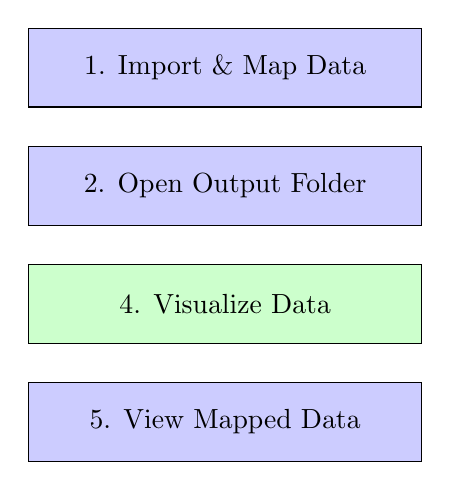
\begin{tikzpicture}
\node[draw, rectangle, fill=blue!20, minimum width=5cm, minimum height=1cm] at (0,0) {1. Import \& Map Data};
\node[draw, rectangle, fill=blue!20, minimum width=5cm, minimum height=1cm] at (0,-1.5) {2. Open Output Folder};
\node[draw, rectangle, fill=green!20, minimum width=5cm, minimum height=1cm] at (0,-3) {4. Visualize Data};
\node[draw, rectangle, fill=blue!20, minimum width=5cm, minimum height=1cm] at (0,-4.5) {5. View Mapped Data};
\end{tikzpicture}
\caption{Button Arrangement (Button 4 highlighted as new feature)}
\end{figure}

\section{Python-Excel Integration}

\subsection{xlwings Library}

\subsubsection{Connection Methods}

\begin{lstlisting}[style=pythonstyle]
import xlwings as xw

# Method 1: Open new instance
app = xw.App(visible=True)
wb = app.books.open("file.xlsx")

# Method 2: Connect to active instance
app = xw.apps.active
wb = app.books[0]

# Method 3: Get caller workbook (from RunPython)
wb = xw.Book.caller()
\end{lstlisting}

\textbf{Our Approach:} Method 1 for standalone, Method 2 when Excel already open

\subsubsection{Reading Data}

\begin{lstlisting}[style=pythonstyle]
# Read single cell
value = sheet.range("A1").value

# Read range
values = sheet.range("A1:C10").value  # Returns list of lists

# Read row
row = sheet.range("1:1").value  # Returns list

# Read column  
col = sheet.range("A:A").value  # Returns list

# Dynamic range
region = sheet.range("A1").current_region.value

# Expand from cell
expanded = sheet.range("A1").expand("table").value
\end{lstlisting}

\subsubsection{Writing Data}

\begin{lstlisting}[style=pythonstyle]
# Write single value
sheet.range("A1").value = "Hello"

# Write list (horizontal)
sheet.range("A1").value = [1, 2, 3]

# Write list (vertical)
sheet.range("A1").options(transpose=True).value = [1, 2, 3]

# Write 2D array
data = [[1, 2], [3, 4], [5, 6]]
sheet.range("A1").value = data

# Batch write (efficient)
sheet.range((1, 1), (3, 2)).value = data
\end{lstlisting}

\subsection{Mapping GUI Implementation}

\subsubsection{GUI Layout}

\begin{figure}[H]
\centering
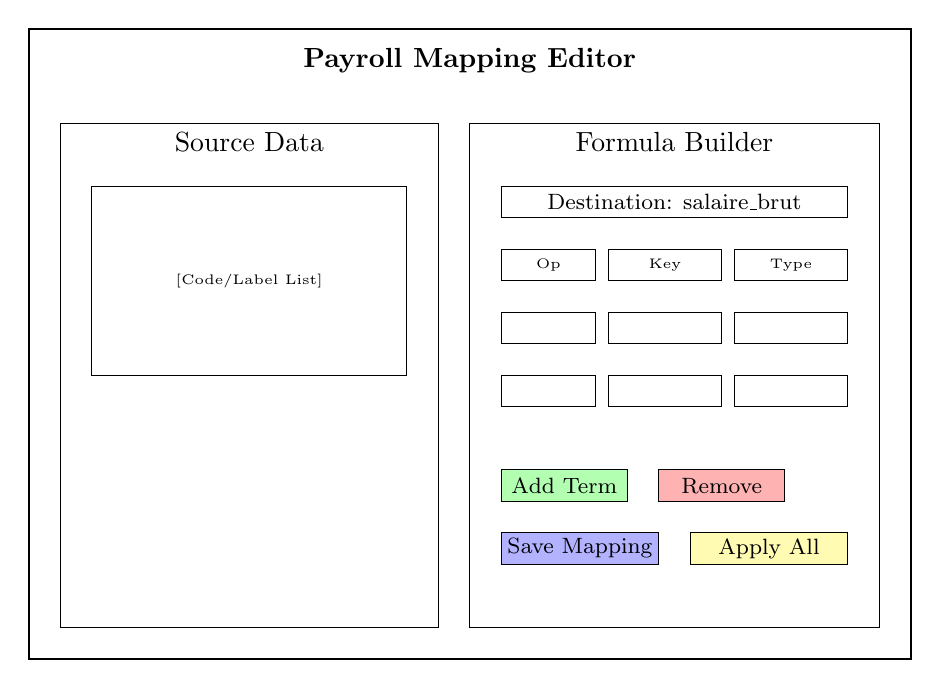
\begin{tikzpicture}[scale=0.8]
% Main window
\draw[thick] (0,0) rectangle (14,10);

% Title
\node at (7,9.5) {\textbf{Payroll Mapping Editor}};

% Left panel - source data
\draw (0.5,0.5) rectangle (6.5,8.5);
\node at (3.5,8.2) {Source Data};
\draw (1,7.5) rectangle (6,4.5);
\node[font=\tiny] at (3.5,6) {[Code/Label List]};

% Center panel - formula builder
\draw (7,0.5) rectangle (13.5,8.5);
\node at (10.25,8.2) {Formula Builder};

% Destination dropdown
\draw (7.5,7.5) rectangle (13,7);
\node[font=\footnotesize] at (10.25,7.25) {Destination: salaire\_brut};

% Formula terms
\foreach \y in {6.5,5.5,4.5} {
    \draw (7.5,\y-0.5) rectangle (9,\y);
    \draw (9.2,\y-0.5) rectangle (11,\y);
    \draw (11.2,\y-0.5) rectangle (13,\y);
}
\node[font=\tiny] at (8.25,6.25) {Op};
\node[font=\tiny] at (10.1,6.25) {Key};
\node[font=\tiny] at (12.1,6.25) {Type};

% Buttons
\draw[fill=green!30] (7.5,2.5) rectangle (9.5,3);
\node[font=\footnotesize] at (8.5,2.75) {Add Term};

\draw[fill=red!30] (10,2.5) rectangle (12,3);
\node[font=\footnotesize] at (11,2.75) {Remove};

\draw[fill=blue!30] (7.5,1.5) rectangle (10,2);
\node[font=\footnotesize] at (8.75,1.75) {Save Mapping};

\draw[fill=yellow!30] (10.5,1.5) rectangle (13,2);
\node[font=\footnotesize] at (11.75,1.75) {Apply All};

\end{tikzpicture}
\caption{Mapping GUI Layout (tkinter)}
\end{figure}

\subsubsection{GUI Code Structure}

\begin{lstlisting}[style=pythonstyle]
def launch_mapping_gui(target_wb, source_path):
    # Create main window
    root = tk.Tk()
    root.title("Payroll Mapping Editor")
    root.geometry("1200x700")
    
    # Open source workbook
    source_wb = target_wb.app.books.open(source_path)
    
    # Get first month sheet
    month_sheets = get_month_sheets(source_wb)
    first_sheet = source_wb.sheets[month_sheets[0]]
    
    # Build GUI components
    # 1. Source data list (left panel)
    source_rows = get_source_rows_display(first_sheet, label_col=2)
    source_listbox = tk.Listbox(root)
    for display, code, label in source_rows:
        source_listbox.insert(tk.END, display)
    
    # 2. Destination dropdown (top center)
    dest_labels = get_all_destination_labels(target_wb, DEST_HEADERS)
    dest_var = tk.StringVar()
    dest_dropdown = ttk.Combobox(root, textvariable=dest_var,
                                 values=dest_labels)
    
    # 3. Formula builder (center)
    formula_frame = ttk.Frame(root)
    term_widgets = []  # List of (operator, key, type) widgets
    
    # 4. Action buttons (bottom)
    def on_add_term():
        # Add new formula term
        pass
    
    def on_save():
        # Save current mapping
        dest = dest_var.get()
        terms = [(op.get(), key.get(), typ.get()) 
                 for op, key, typ in term_widgets]
        save_mapping_row(source_wb, dest, terms)
        messagebox.showinfo("Saved", f"Mapping saved for {dest}")
    
    def on_apply_all():
        # Apply all saved mappings
        root.destroy()  # Close GUI
        apply_mappings_from_source(source_wb, target_wb)
    
    ttk.Button(root, text="Add Term", 
               command=on_add_term).pack()
    ttk.Button(root, text="Save Mapping", 
               command=on_save).pack()
    ttk.Button(root, text="Apply All", 
               command=on_apply_all).pack()
    
    # Start GUI loop
    root.mainloop()
\end{lstlisting}

\subsubsection{Dynamic Label Creation}

\begin{lstlisting}[style=pythonstyle]
def add_new_label():
    """Allow user to create custom destination label."""
    dialog = tk.Toplevel(root)
    dialog.title("Add Custom Label")
    
    tk.Label(dialog, text="Enter new label name:").pack()
    entry = tk.Entry(dialog)
    entry.pack()
    
    def on_ok():
        new_label = entry.get().strip()
        if not new_label:
            messagebox.showwarning("Empty", "Please enter a label")
            return
        
        # Add to destination dropdown
        current_values = list(dest_dropdown['values'])
        if new_label not in current_values:
            current_values.append(new_label)
            dest_dropdown['values'] = current_values
            dest_var.set(new_label)
        
        dialog.destroy()
    
    tk.Button(dialog, text="OK", command=on_ok).pack()
    tk.Button(dialog, text="Cancel", 
              command=dialog.destroy).pack()
\end{lstlisting}

\subsection{Automatic Execution}

\begin{lstlisting}[style=pythonstyle]
def launch_mapping_gui(target_wb, source_path):
    # ... GUI code ...
    
    def on_apply_all():
        # Track which labels were modified
        modified_labels = list(modified_labels_set)
        
        # Close GUI
        root.destroy()
        
        # Automatically apply mappings (no separate button needed)
        try:
            apply_mappings_from_source(
                source_wb, target_wb,
                modified_labels_only=modified_labels
            )
        except Exception as e:
            messagebox.showerror("Error", str(e))
\end{lstlisting}

\textbf{Key Innovation:} When GUI closes, mappings apply automatically. User doesn't need to:
\begin{itemize}
    \item Save workbook
    \item Run separate script
    \item Click another button
\end{itemize}

Everything happens seamlessly.
